\section{Yields}

\subsection{Fit procedure}
 The yields of signal and background events in the data are
 determined in the mass range 5.35--6.00\gevcc using unbinned
 extended maximum likelihood fits for the \decay{\Lb}{\Lz\mumu} and
 the \decay{\Lb}{\jpsi\Lz} modes.  The likelihood function has the form
\begin{equation}
\mathcal{L}=e^{-(N_\mathrm{S}+N_\mathrm{C}+N_{\mathrm{P}})} \times \prod_{i=1}^{N}[
  N_\mathrm{S}P_{\mathrm{S}}(m_i)+N_\mathrm{C}P_\mathrm{C}(m_i)+N_{\mathrm{P}}P_{\mathrm{P}}(m_i)]
 \;,
\label{eq:uml}
\end{equation}
 \noindent where $N_\mathrm{S}$, $N_\mathrm{C}$ and $N_\mathrm{P}$ are
 the number of
 signal, combinatorial and peaking background events, respectively, 
 $P_j(m_i)$ are the corresponding probability density functions
 (PDFs) and $m_i$  is the mass of the \Lb candidate. 
 The signal yield itself is parametrised in the fit using the
 relative branching fraction of the signal and normalisation modes,
%
\begin{equation}
N_\mathrm{S}(\Lz\mumu)_{k}  = \left[ \frac{\mathrm{d}\mathcal{B}(\Lz\mumu)/\mathrm{d}\qsq}{\mathcal{B}(\jpsi\Lz)} \right]  \cdot
N_\mathrm{S}(\jpsi\Lz)_{k} \cdot \varepsilon^{\mathrm{rel}}_{k} \cdot \frac {\Delta\qsq} { \mathcal{B}(\jpsi\to\mumu) },
\label{eq:ield_from_BR}
\end{equation}
\noindent
where $k$ is the candidate category (long or downstream), $\Delta\qsq$
is the width of the \qsq interval considered and
$\varepsilon_k^{\mathrm{rel}}$ is the relative efficiency, fixed to
the values obtained as described in Sec.~\ref{sec:efficiency}. Fitting
the ratio of the branching fractions of signal and normalisation modes
simultaneously in both candidate categories makes better statistical
use of the data.

 The signal shape, in both \decay{\Lb}{\Lz\mumu} and
 \decay{\Lb}{\jpsi\Lz} modes, is described by the sum of two Crystal
 Ball functions~\cite{Skwarnicki:1986xj} that share common means and
 tail parameters but have independent widths.  The combinatorial
 background is parametrised by an exponential function, independently
 in each \qsq interval. The background due to \decay{\Bz}{\jpsi\KS}
 decays is modelled by the sum of two Crystal Ball functions with
 opposite tails. All shape parameters are independent
 for the downstream and long sample.

 For the \decay{\Lb}{\jpsi\Lz} mode, the widths and common mean in the
 signal parametrisation are free parameters. The parameters describing
 the shape of the peaking background are fixed to those derived from
 simulated \decay{\Bz}{\jpsi\KS} decays, with only the normalisation
 allowed to vary to accomodate differences between data and simulation.

 For the \decay{\Lb}{\Lz\mumu} decay, the signal shape parameters are
 fixed according to the result of the fit to \decay{\Lb}{\jpsi\Lz}
 data and the widths are rescaled to allow for possible differences
 in resolution as a function of \qsq. The scaling factor is determined
 comparing \decay{\Lb}{\jpsi\Lz} and \decay{\Lb}{\Lz\mumu} simulated events.
 %The ratio between the widths of the two Crystal Ball functions 
 %summed to obtain the signal PDF is constrained to
 %that obtained from the normalisation mode, with a common scale
 %factor, determined from a fit to simulated \decay{\Lb}{\Lz\mumu}
 %events, allowing for possible differences in resolution as a function
 %of \qsq.  
 The \decay{\Bz}{\KS\mumu} background component is also
 modelled using the sum of two Crystal Ball functions with opposite
 tails where both the yield and all shape parameters are constrained
 to those obtained from simulated events.
 
\subsection{Fit results}
 The invariant mass distribution of the \decay{\Lb}{\jpsi\Lz}
 candidates selected with the high-\qsq requirements is shown in
 Fig.~\ref{fig:totalFit}, combining both long and downstream
 candidates.  The normalisation channel candidates are divided into
 four sub-samples: downstream and long events are fitted separately
 and each sample is selected with both the low-\qsq and high-\qsq
 requirements to normalise the corresponding \qsq regions in signal.
 The number of \decay{\Lb}{\jpsi\Lz} decays found in each case
 is given in Table~\ref{tab:jpsi_yield}.
%
\begin{table}[tbp]
\centering
\caption{Number of \decay{\Lb}{\jpsi\Lz} decays in the long and
  downstream categories found using the selection for low- and
  high-\qsq regions. Uncertainties shown are statistical only.}
\begin{tabular}{lcc}
Selection & $N_{\rm S}$ (long) & $N_{\rm S}$ (downstream)\\ \hline
high-\qsq	& $4313 \pm 70$	 	&  $11\,497 \pm 123$ \\
low-\qsq	& $3363 \pm 59$ 	&  $\phantom{0}\,7225 \pm 89\phantom{0}$  \\
 \hline
\end{tabular}
\label{tab:jpsi_yield}
\end{table}
%
\begin{figure}[tpbh!]
%%\centering \includegraphics[width=0.8\textwidth]{images_and_tables/BR/fit_Jpsi_All_log.pdf}
\centering 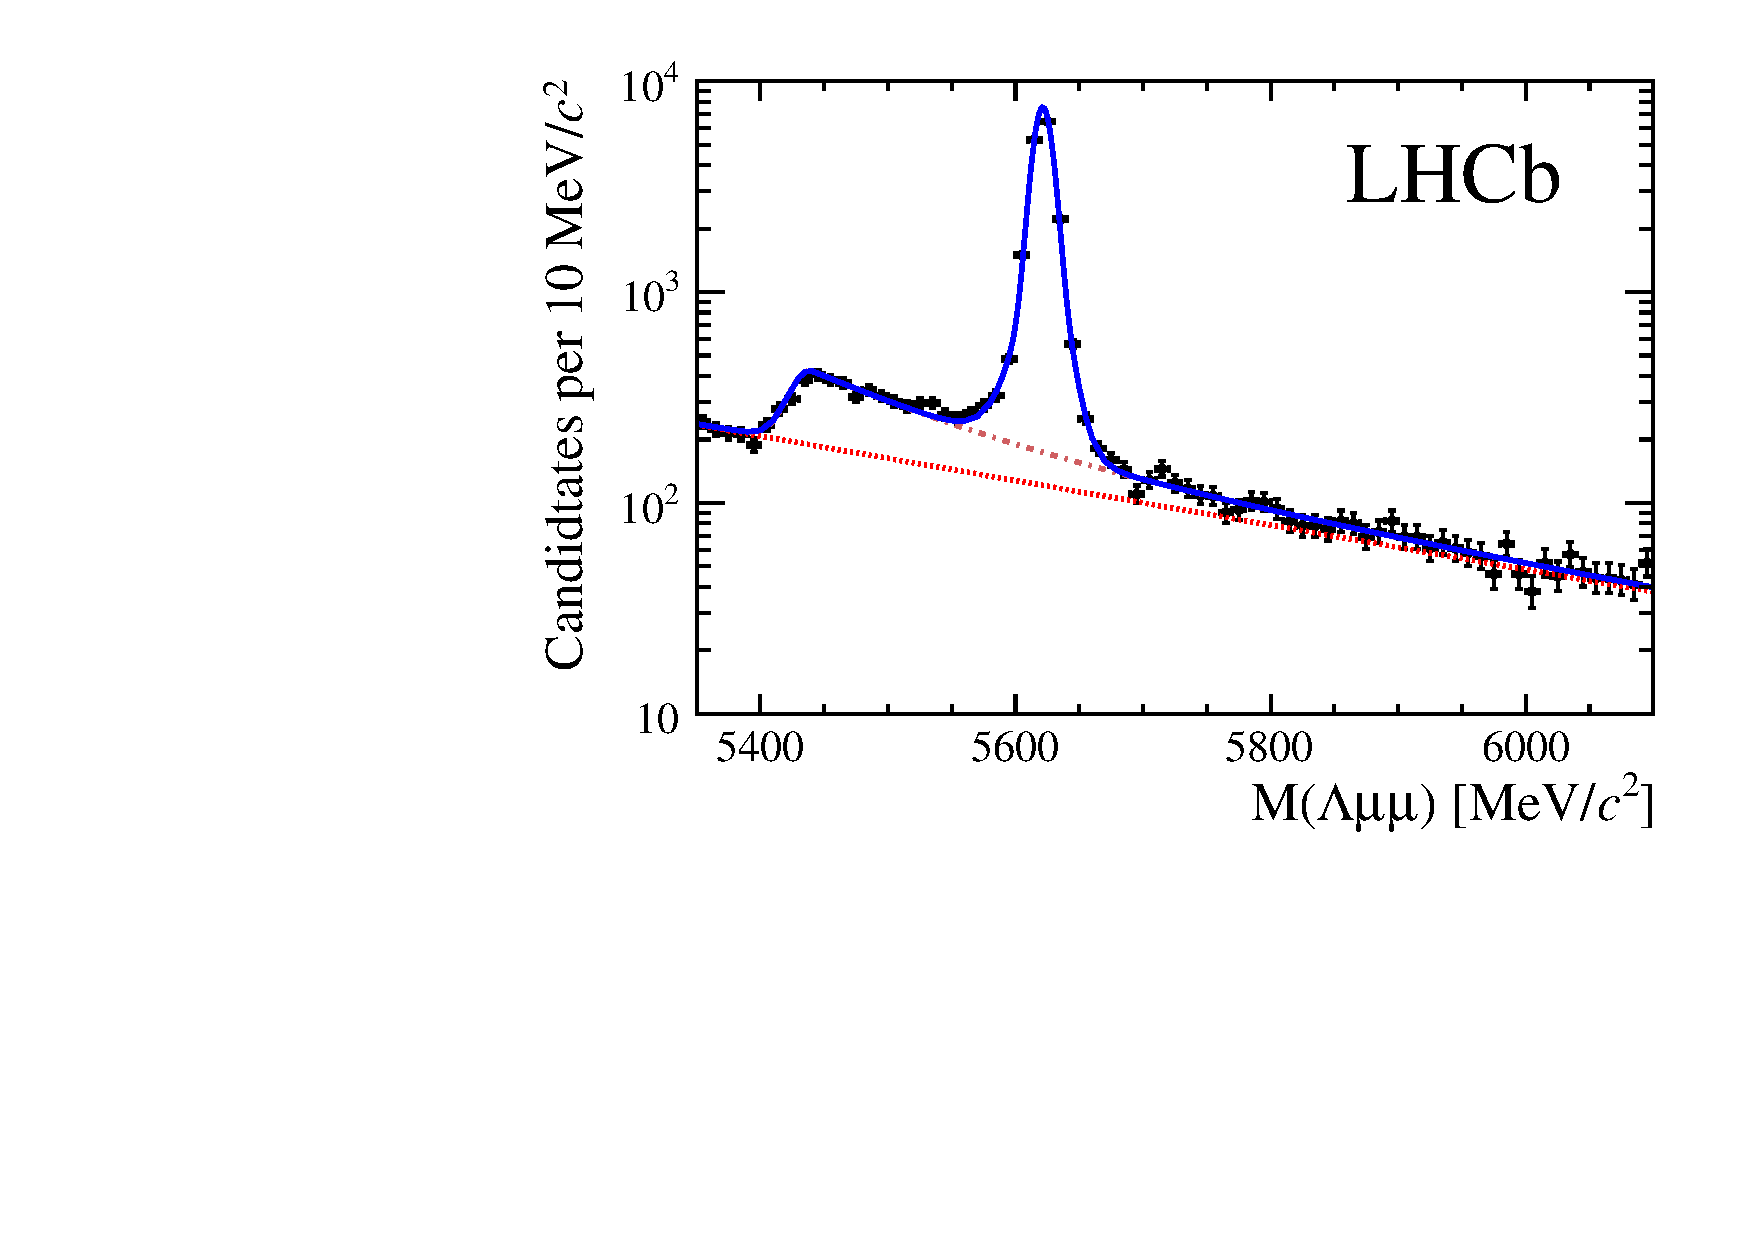
\includegraphics[width=0.8\textwidth]{figure1.pdf}
\caption{\small Invariant mass distribution of the \decay{\Lb}{\jpsi\Lz}
  candidates selected with the neural network requirement used for the high-\qsq region.
  The (black) points show data, combining downstream
  and long candidates, and the solid (blue) line represents the
  overall fit function.  The dotted (red) line represents the combinatorial
  and the dash-dotted (brown) line the peaking background from
  \decay{\Bz}{\jpsi\KS} decays.}
\label{fig:totalFit}
\end{figure}

  The fraction of peaking background events is larger in the
  downstream sample amounting to 28\,\% of the \decay{\Lb}{\jpsi\Lz} yield in the
  full fitted mass range, while in the sample of long candidates it
  constitutes about 4\,\%.

  The invariant mass distributions for the \decay{\Lb}{\Lz\mumu}
  process, integrated over $15.0<\qsq<20.0$\gevgevcccc and in eight
  separate \qsq intervals, are shown in Figs.~\ref{fig:totalFitRare}
  and \ref{fig:differentialFit}.  The yields found in each \qsq
  interval are given in Table~\ref{tab:rareYields} together with their
  significances.  The statistical significance of the observed signal
  yields is evaluated as $\sqrt{2\Delta\ln{\mathcal{L}}}$, where
  $\Delta\ln{\mathcal{L}}$ is the change in the logarithm of the
  likelihood function when the signal component is excluded from the
  fit, relative to the nominal fit in which it is present.

\begin{figure}[tbph!]
%%\centering \includegraphics[width=0.8\textwidth]{images_and_tables/BR/fit_All_highQ2.pdf}
\centering 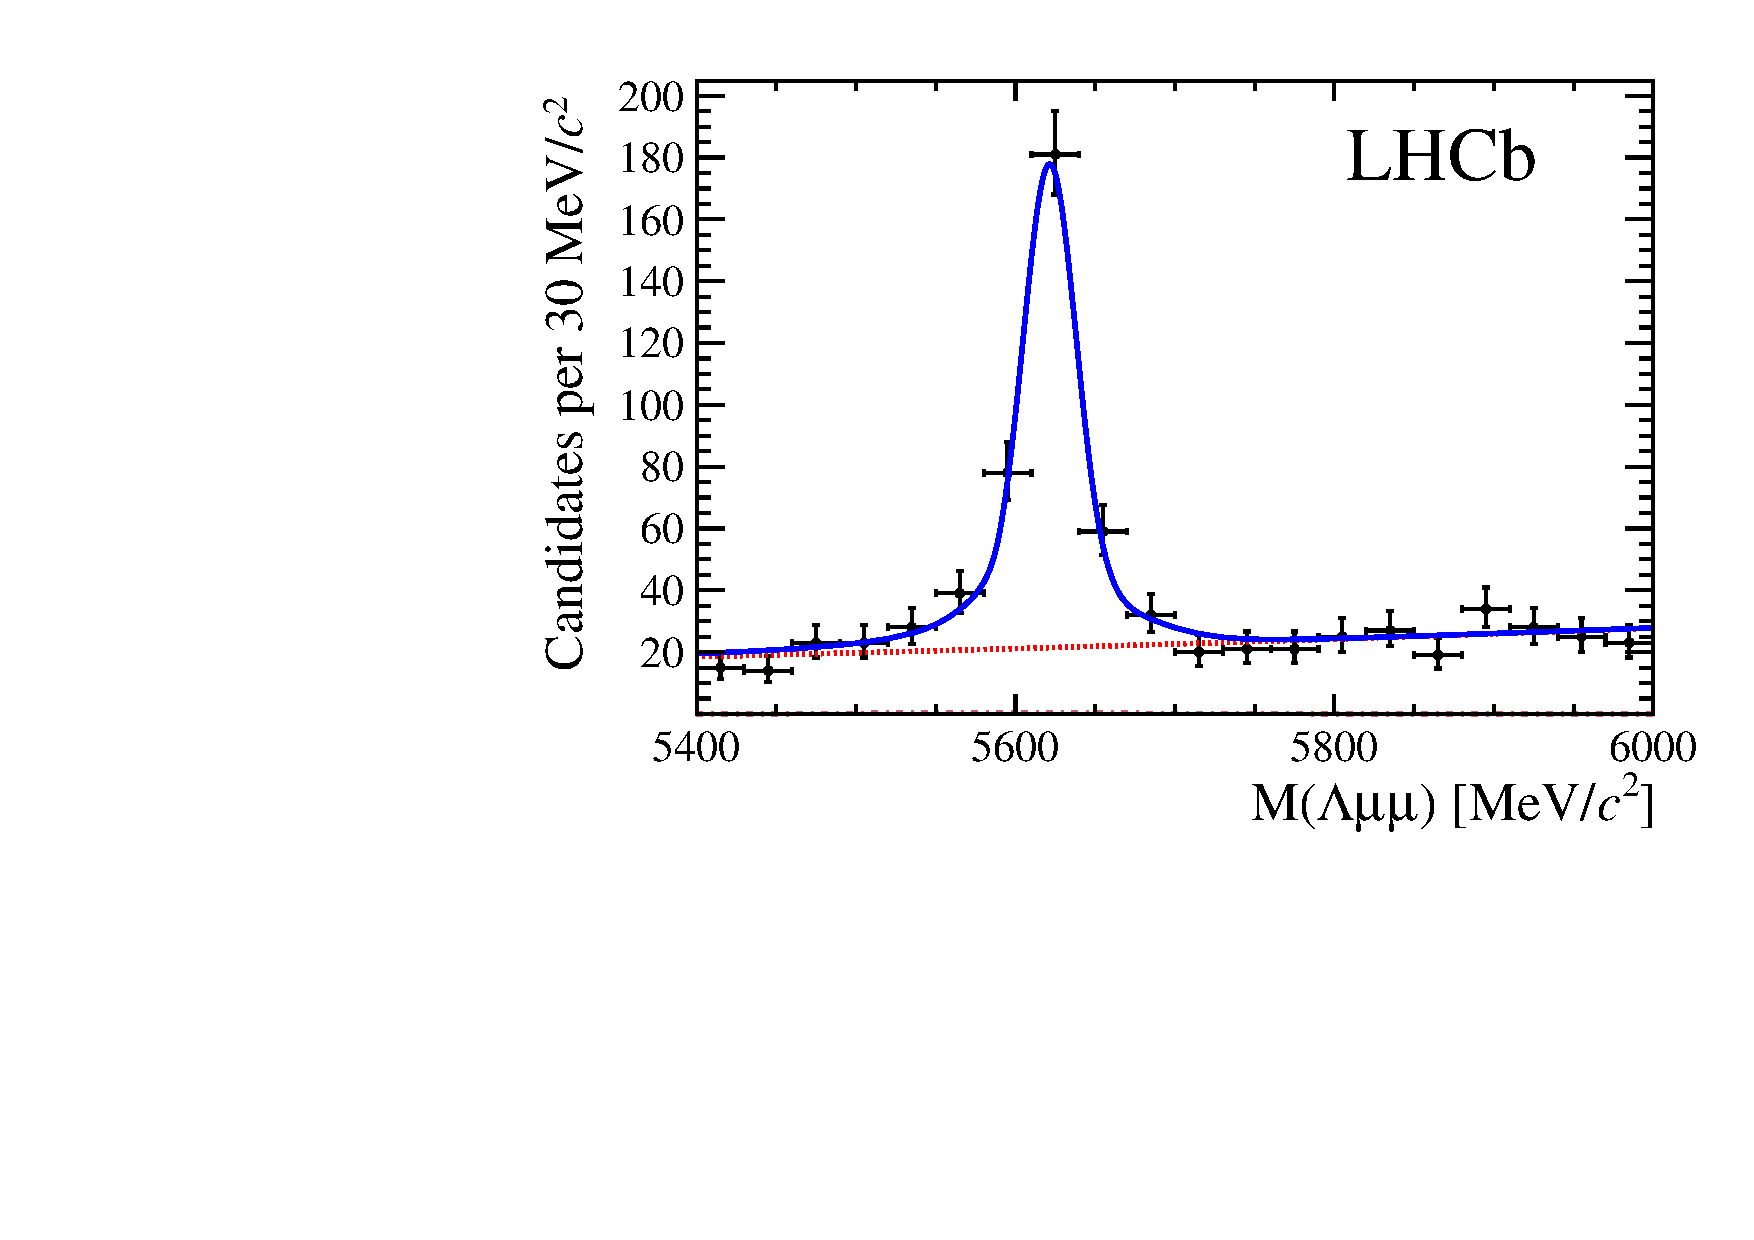
\includegraphics[width=0.8\textwidth]{figure2.pdf}
\caption{\small Invariant mass distribution of the
  \decay{\Lb}{\Lz\mumu} candidates, integrated over the region  $15.0 < \qsq < 20.0$ \gevgevcccc 
  together with the fit function described in the text.  The points show data,
  the solid (blue) line is the overall fit function and the dotted
  (red) line represents the combinatorial background.
  The background component from \decay{\Bz}{\KS\mumu} decays, (brown)
  dashed line, is barely visibile due to the very low yield.}
\label{fig:totalFitRare}
\end{figure}
%
\begin{figure}[tbph]
%%\centering \includegraphics[width=0.64\textheight]{images_and_tables/BR/q2_fits_All_vertical.pdf}
\centering 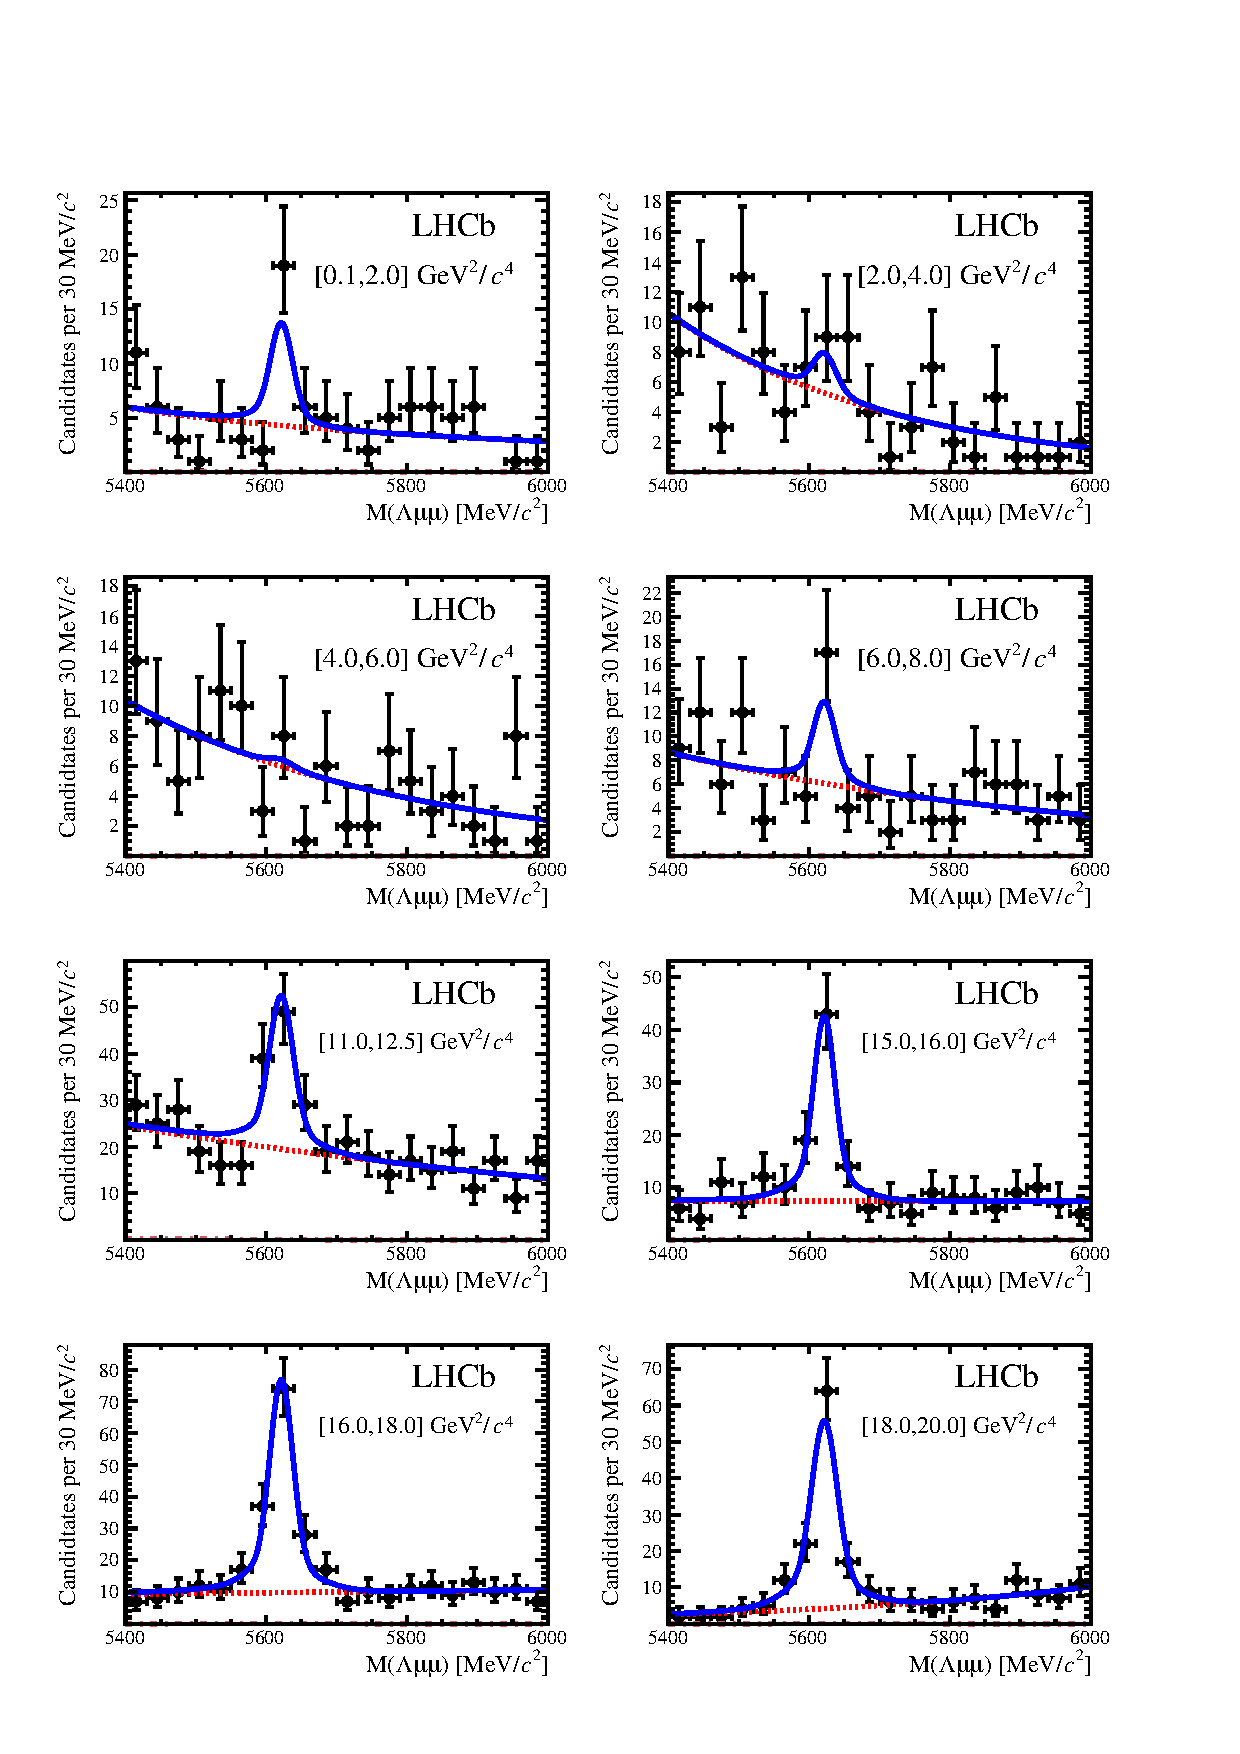
\includegraphics[width=0.64\textheight]{figure3.pdf}
\caption{\small Invariant mass distributions of \decay{\Lb}{\Lz\mumu}
candidates, in eight \qsq\ intervals, together with the
  fit function described in the text. The points show data, the
  solid (blue) line is the overall fit function and
  the dotted
  (red) line represents the combinatorial background component.}
\label{fig:differentialFit}
\end{figure}
%
\begin{table}[btph!]
\centering
\caption{\small Signal decay yields ($N_\mathrm{S}$) obtained from the
  mass fit to \decay{\Lb}{\Lz\mumu} candidates in each \qsq interval
  together with their statistical significances. 
  The yields are the sum of long and downstream categories with
  downstream decays comprising $\sim 80\,\%$ of the total yield.
  The $8-11$ and $12.5-15$ \gevgevcccc ~\qsq intervals are excluded
  from the study as they are dominated by decays via charmonium resonances.
  }
\label{tab:rareYields}
\begin{tabular}{ccc}
 $q^2$ interval [\gevgevcccc] & Total signal yield & Significance \\ \hline
0.1 -- 2.0    &  $16.0\pm5.3$            &  4.4 \\
2.0 -- 4.0    &  $\phantom{0}4.8\pm4.7$  &  1.2 \\
4.0 -- 6.0    &  $\phantom{0}0.9\pm2.3$  &  0.5 \\
6.0 -- 8.0    &  $11.4\pm5.3$            &  2.7 \\
11.0 -- 12.5  &  $\phantom{.0}60\pm12\phantom{.}$           &  6.5 \\
15.0 -- 16.0  &  $57\pm9$                &  8.7 \\
16.0 -- 18.0  &  $118\pm13$              &  13  \\
18.0 -- 20.0  &  $\phantom{.}100\pm11\phantom{.}$   &  14  \\
\hline
1.1 -- 6.0    &  $\phantom{0}9.4\pm6.3$  &  1.7 \\
15.0 -- 20.0  &  $276\pm20$              &  21  \\
\end{tabular}  
\end{table}

%\clearpage

